\chapter{基于压缩后缀数组的序列比对算法}
本章将介绍基于CSA的短读比对算法(CSAA)。CSAA采用CSA索引参考序列,利用CSA的后向搜索完成匹配过程。CSA的后向搜索是一种精确匹配
算法,可以在$O(m\log n)$是间复杂度内找出长为$m$的模式$P$在长为$n$的序列中的后缀数组位置。然而,由于DNA序列存在个体变异,以及测
序技术有一定的错误率,反应在短读序列上就是短读序列的每一个核苷酸并非都是可靠的,所以在做短读映射时就不能简单的使用精确模式匹配
算法,而应该尽可能根据短读序列的性质找到一个最可靠的匹配位置。本文提出了两种策略来实现短读比对中的非精确匹配
要求。一是在后向搜索过程中引入了搜索树,使得在短读匹配过程中可以随时对短读序列上的某个核苷酸进行插入,删除,替换等操作,达到模
糊匹配的目的。另一个策略是在搜索树上引入优先堆的数据结构,这一数据结构结合评分机制保证在后向搜索的每一步中都是沿着最优的搜索
方向前进,并且采用分支限界的策略适时淘汰很差的搜索方向,最终实现找到一个最优的匹配位置的目的。

\section{精确匹配}
精确匹配本质上就是是后向搜索。根据算法\ref{alg:backwardsearch},可知给定一个长为$n$的参考序列$T$,$P$为测序得到的短读序列中的
一个短读,假设已经获取到短读的后缀$P[i+1\ldots m-1]$的后缀数组位置$(l_{P_{i+1}},r_{P_{i+1}})$,那么可以跟据公式\ref{equa:exac}
确定后缀$P[i\ldots m-1]$的后缀数组位置$(l_{P_i},r_{P_i})$。

\begin{equation}\label{equa:exac}
    \begin{split}
        l_{P_i} \gets &\min\{ k \in [\alpha(P[i]),\alpha(P[i])+\beta(P[i])-1],\Phi[k] \in [l_{P_{i+1}},r_{P_{i+1}]}\}\\
        r_{P_i} \gets &\max\{ k \in [\alpha(P[i]),\alpha(P[i])+\beta(P[i])-1],\Phi[k] \in [l_{P_{i+1}},r_{P_{i+1}]}\}
    \end{split}
\end{equation}

由于$\Phi[\alpha(P[i])\ldots \alpha(P[i])+\beta(P[i])-1]$是严格递增序列,所以公式\ref{equa:exac}可以采用二分搜索实现。
搜索$[\alpha(P[i],\alpha(P[i])+\beta(P[i])-1]$的
左边界和右边界在$\Phi[\alpha(P[i])\ldots \alpha(P[i])+\beta(P[i])-1]$上是否出现,即可得$P[i\ldots n-1]$的后缀数组
位置$(l_{P_i},r_{P_i})$。

综上所述,可以得到以下精确匹配算法\ref{alg:exac},该算法采用后向搜索的方法,根据一个给定的模式$X$的后缀数组$(l,r)$和
字符$c$计算出新模式$cX$的后缀数组位置。根据这个算法,加上一定策略,即可得到我们下文将提出的近似匹配算法。

\begin{algorithm}
    \caption{精确匹配}
    \label{alg:exac}
    \begin{algorithmic}[1]
        \Require $\Phi,\alpha,\beta,l_{old},r_{old},c$
        \Ensure $(l,r)$
        \Function{ExactMatch}{$\Phi,\alpha,\beta,l_{old},r_{old},c$}
        \State $l_c \gets \alpha(c)$
        \State $r_c \gets \alpha(c)+\beta(c)-1$
        \State $(l,r) \gets $\Call{binarySearch}{$\Phi[l_c\ldots r_c],l_{old},r_{old}$}
        \If{$l>r$}
            \State \Return $\varnothing$
        \Else
            \State \Return $(l,r)$
        \EndIf
        \EndFunction
    \end{algorithmic}
\end{algorithm}

\section{近似匹配}

根据上一小节所述的精确匹配算法思想,模式匹配就只有两种结果,要么匹配上,要么没匹配上这种完全的匹配方式并不适合大多数存在变异
和测序误差的短读序列。本文提出的CSAA算法是建立在非精确匹配的基础上的。

由于同一物种之间存在的个体差异(具体在DNA上表现为单核苷酸变异SNP),以及测序技术存在的误差,Resequencing技术得到的短读序列和
该物种的标准参考序列之间哪怕是同一基因片段也必然存在着一些不同,这会造成即使同一种基因序列也无法完全比对映射到参考序列上。
所以对短读和参考序列之间的比对仅仅精确比对映射是远远不够的,这会造成大量的短读因为和参考序列相差一两个核苷酸不同而不能映射
到参考序列上,而这一两个不同的核苷酸很可能是测序误差或者生物个体之间的SNP造成的,不应当认为二者是不能匹配的。所以,采用合适
的非精确比对算法是必须的。本文提出的非精确匹配算法中,支持对短读进行替换(substitude),插入(insert),删除(delete)三种变换操
作,通过这三种操作可以保证变异的或者发生测序错误的短读序列依然能正确匹配到参考序列的合适位置上。

考虑一个给定的长为$m$的短读序列$P$,采用后向搜索,当搜索到第$i+1$个位置时,得到序列$P_{i+1}$的后缀数组位置$(l_{i+1},r_{i+1})$,
依照精确匹配的算法下一步应当在$(l_{i+1},r_{i+1})$的基础上搜索字符$P[i]$,从而得到一个新的后缀数组位置$(l_i,r_i)$。在此,如果我们不
搜索$P[i]$,而是搜索另一个符号$c \neq P[i]$,得到另一个后缀数组位置$(l_{i}^{'},r_{i}^{'})$。接着在$(l_{i}^{'},r_{i}^{'})$基础
上继续搜索$P[0\ldots i-1]$,那么最终得到后缀数组位置$(l_0,r_0)$将不再是序列$P$的一个后缀数组位置了,而是将$P[i]$替换为$c$
后的新字符串的后缀数组位置。称这个新位置为$P$的一个替换近似串的后缀数组位置,计为$(l_0,r_0,m,P(S_i))$,即长为$m$的序列$P$在
$i$位置进行一次替换后可以映射到参考序列的后缀数组位置$(l_0,r_0)$。

图\ref{fig:substitude}给出了把短读序列中的一个符号$T$替换为$A$时的搜索过程,实线为精确匹配的过程,虚线是替换后的搜索过程。

\begin{figure}[htbp]
    \centering
    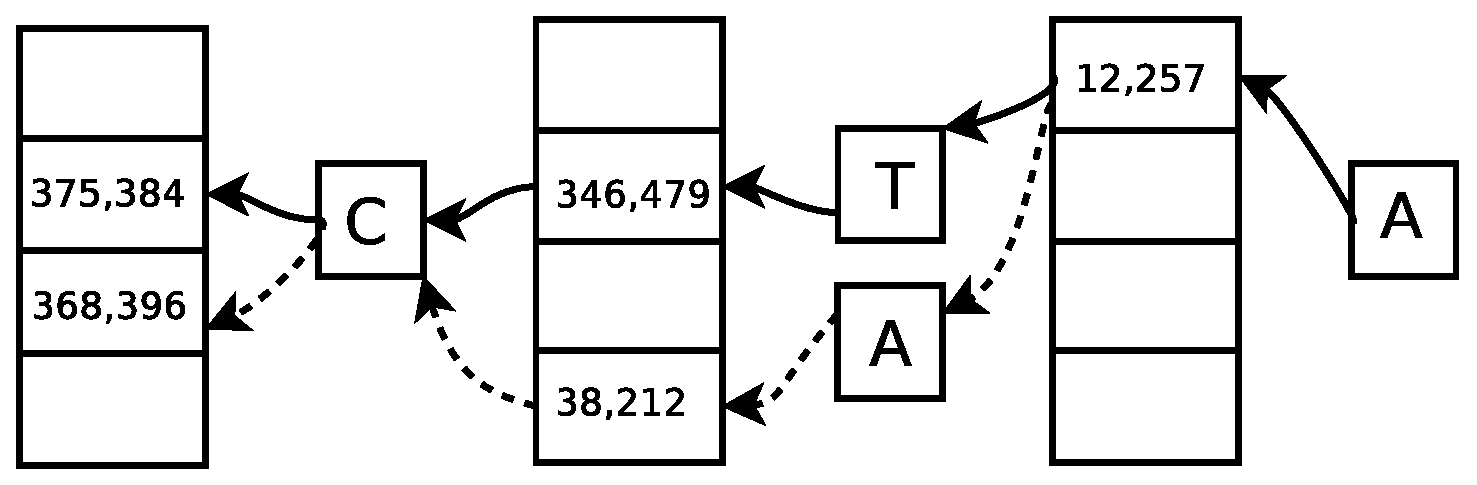
\includegraphics[width=0.7\textwidth]{substitude.eps}
    \caption{替换操作示例} \label{fig:substitude}
\end{figure}

不同于替换操作,如果在搜索到$P[i]$时,放弃搜索$P[i]$符号,直接在$(l_{i+1},r_{i+1})$的基础上搜索序列$P[0\ldots i-1]$,那么
最终得到的后缀数组位置$(l_0,r_0)$将是$P$删除$P[i]$后的近似串在参考序列上的后缀数组位置,计为$(l_0,r_0,m,P(D_i))$,,即长为$m$
的序列$P$在$i$位置进行一次删除后可以映射到参考序列的后缀数组位置$(l_0,r_0)$。

如图\ref{fig:delete}所示为删除短读序列中的一个符号后的搜索过程。

\begin{figure}[htbp]
    \centering
    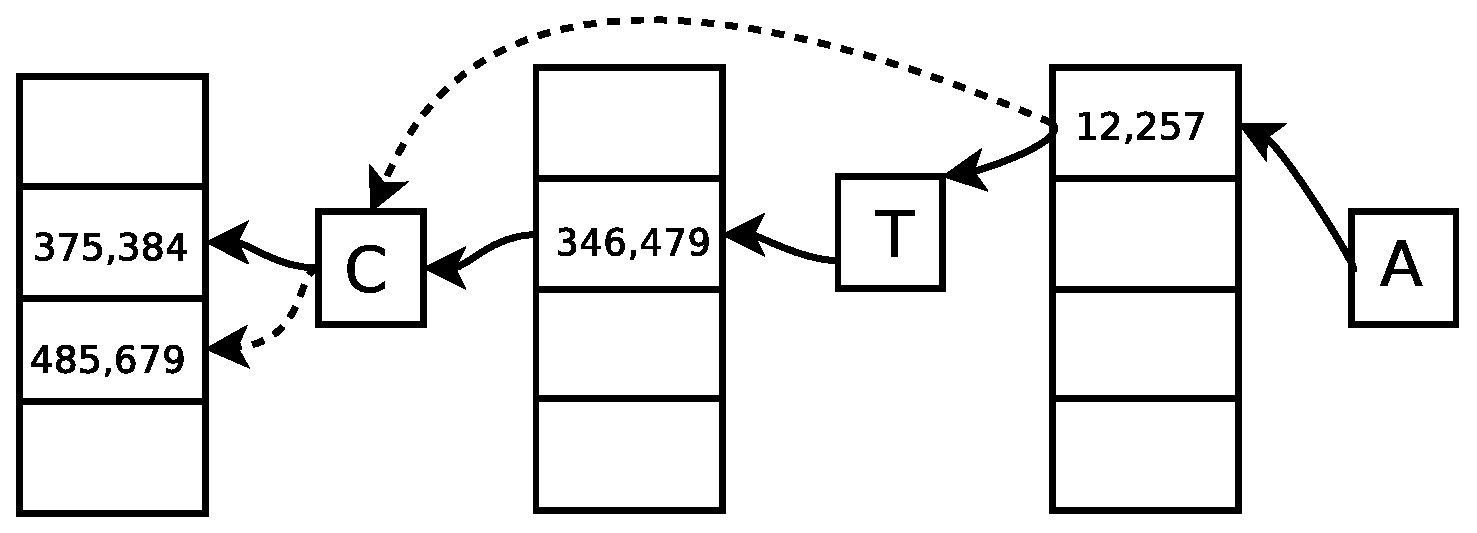
\includegraphics[width=0.7\textwidth]{delete.eps}
    \caption{删除操作示例} \label{fig:delete}
\end{figure}

对于插入操作,在搜索到$P[i]$时,不直接搜索$P[i]$,而是在$l_{i-1},r_{i-1}$的基础上搜索符号$c$,得到$(l_{i}^{'},r_{i}^{'})$,接着
在此基础上搜索序列$P[0\ldots i]$,最终得到的后缀数组位置$(l_0,r_0)$将是$P$在$i$位置插入符号$c$后的近似序列的后缀数组位置。计为
$(l_0,r_0,m,P(Ii)$,即长为$m$的序列$P$在$i$位置插入一个符号后可以映射到参考序列的后缀数组位置$(l_0,r_0)$。

如图\ref{fig:insert}所示为插入一个符号'A'前后的短读序列中的一个符号后的搜索过程。

\begin{figure}[htbp]
    \centering
    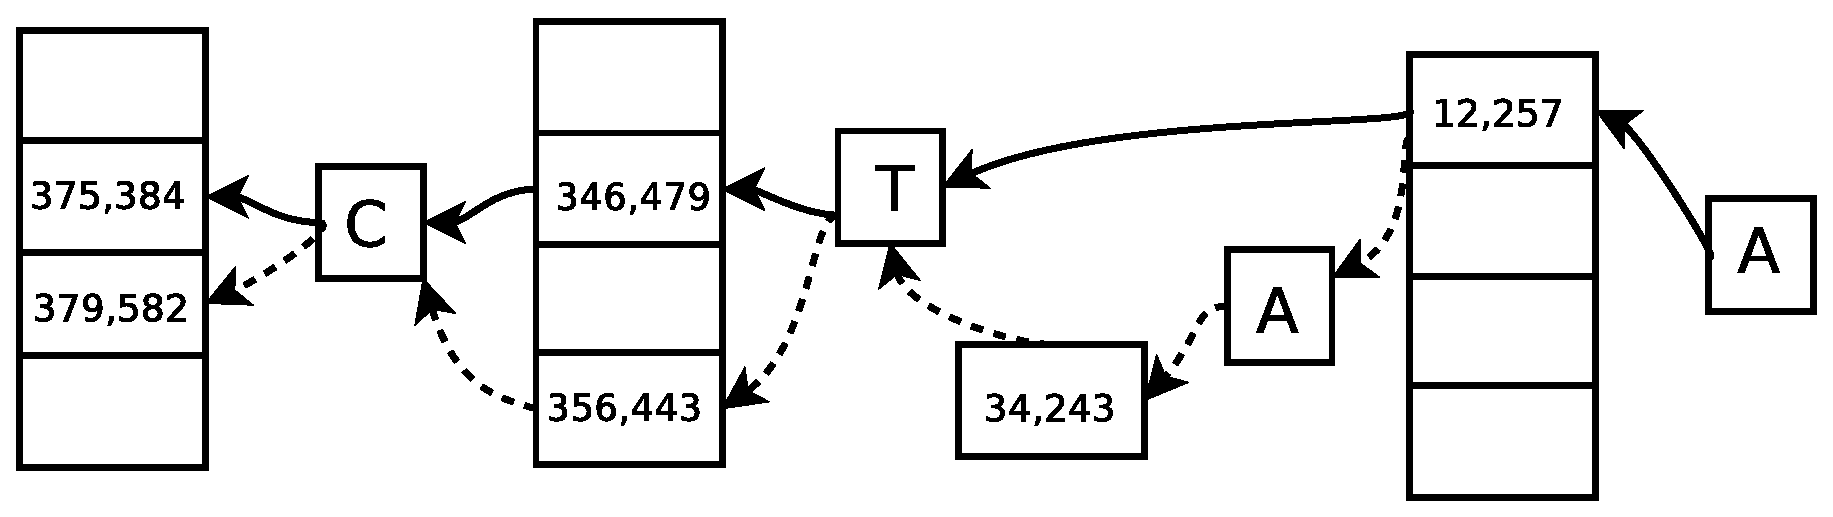
\includegraphics[width=0.7\textwidth]{insert.eps}
    \caption{插入操作示例} \label{fig:insert}
\end{figure}

综上所述,通过在搜索的过程中加入替换,删除,插入三种操作,可以扩展后向搜索的搜索方向,达到近似匹配的目的。如果已知模式串的
某个字符是不可靠的,那么我们可以通过在这个位置加入上述三种操作,实现非精确匹配,查找到这个模式串的可能匹配位置。而大多数情况
下,我们是不知道具体哪一个字符不可靠的,所以只能试探每一个字符,对每一个字符都做删除,替换,插入操作,从而找到一个合适的位置。
据此,我们提出非精确匹配算法\ref{alg:inexact},这个算法递归的实现近似匹配,对$P$的每一个位置都做了三种操作,所以这个算法的本
质是对长为$m$的序列$m$做了所有可能的近似串的搜索,即做了$|\Sigma|^m$个序列的匹配。因为采用了后向搜索的过程,每一次递归实际都
是产生$\Sigma$次替换递归,$\Sigma$次插入递归,和1次删除递归,所以实际的时间复杂度
满足递归式\ref{equa:exact}。解递归式\ref{equa:exact}可得$T(m)=(2\Sigma+1)^{m-1}+\Theta(m\log n)$。
\begin{equation}\label{equa:exact}
    T(m)=\begin{cases}\Theta(1) & \mbox{if } m=1 \\
    2(\Sigma+1)T(m-1)+\Theta(\log n) & \mbox{if } m>1\end{cases}
\end{equation}

\begin{algorithm}
    \caption{近似匹配}
    \label{alg:inexact}
    \begin{algorithmic}[1]
    \Require $\Phi,\alpha,\beta,l,r,P,i$
    \Ensure $(l,r)$
    \Function{inexactMatch}{$\Phi,\alpha,\beta,l,r,P,i$}
    \If{$i<0$}
    \State \Return $(l,r)$
    \EndIf
    \State $S \gets \varnothing$
    \State $S \gets S\ \cup$\ \Call{inexactMatch}{$\Phi,\alpha,\beta,l,r,P,i-1$} \Comment{删除$P[i]$操作}
    \ForAll{$c \in \Sigma$}
    \State $(l,r)\gets$\Call{ExacMatch}{$\Phi,\alpha,\beta,l,r,c$} \Comment{调用算法\ref{alg:exac}}
        \If{$l\leq r$}
        \State $S \gets S\ \cup\ $ \Call{inexactMatch}{$\Phi,\alpha,\beta,l,r,P,i-1$} \Comment{替换$P[i]$为$c$}
        \State $S \gets S\ \cup\ $ \Call{inexactMatch}{$\Phi,\alpha,\beta,l,r,P,i$} \Comment{在$P[i]$后插入$c$}
        \EndIf
    \EndFor
    \State \Return $S$
    \EndFunction
\end{algorithmic}
\end{algorithm}

\section{搜索树}

根据上一小节中描述的方法,用后向搜索实现替换,删除,插入操作的方法,实现短读序列的近似匹配。在不知道具体的替换,删除以及插入
位置时,需要在每一次后向搜索一个符号时都分别做一次替换,删除,插入操作。而每一次操作实际上都导致了一个新的近似序列的产生,在
未完成整个序列的搜索时,最终哪一个近似序列能够较好的映射到参考序列上依然是未知的,这就要求我们在搜索过程中保留每一个可能的近
似序列。

\begin{figure}[htbp]
    \centering
    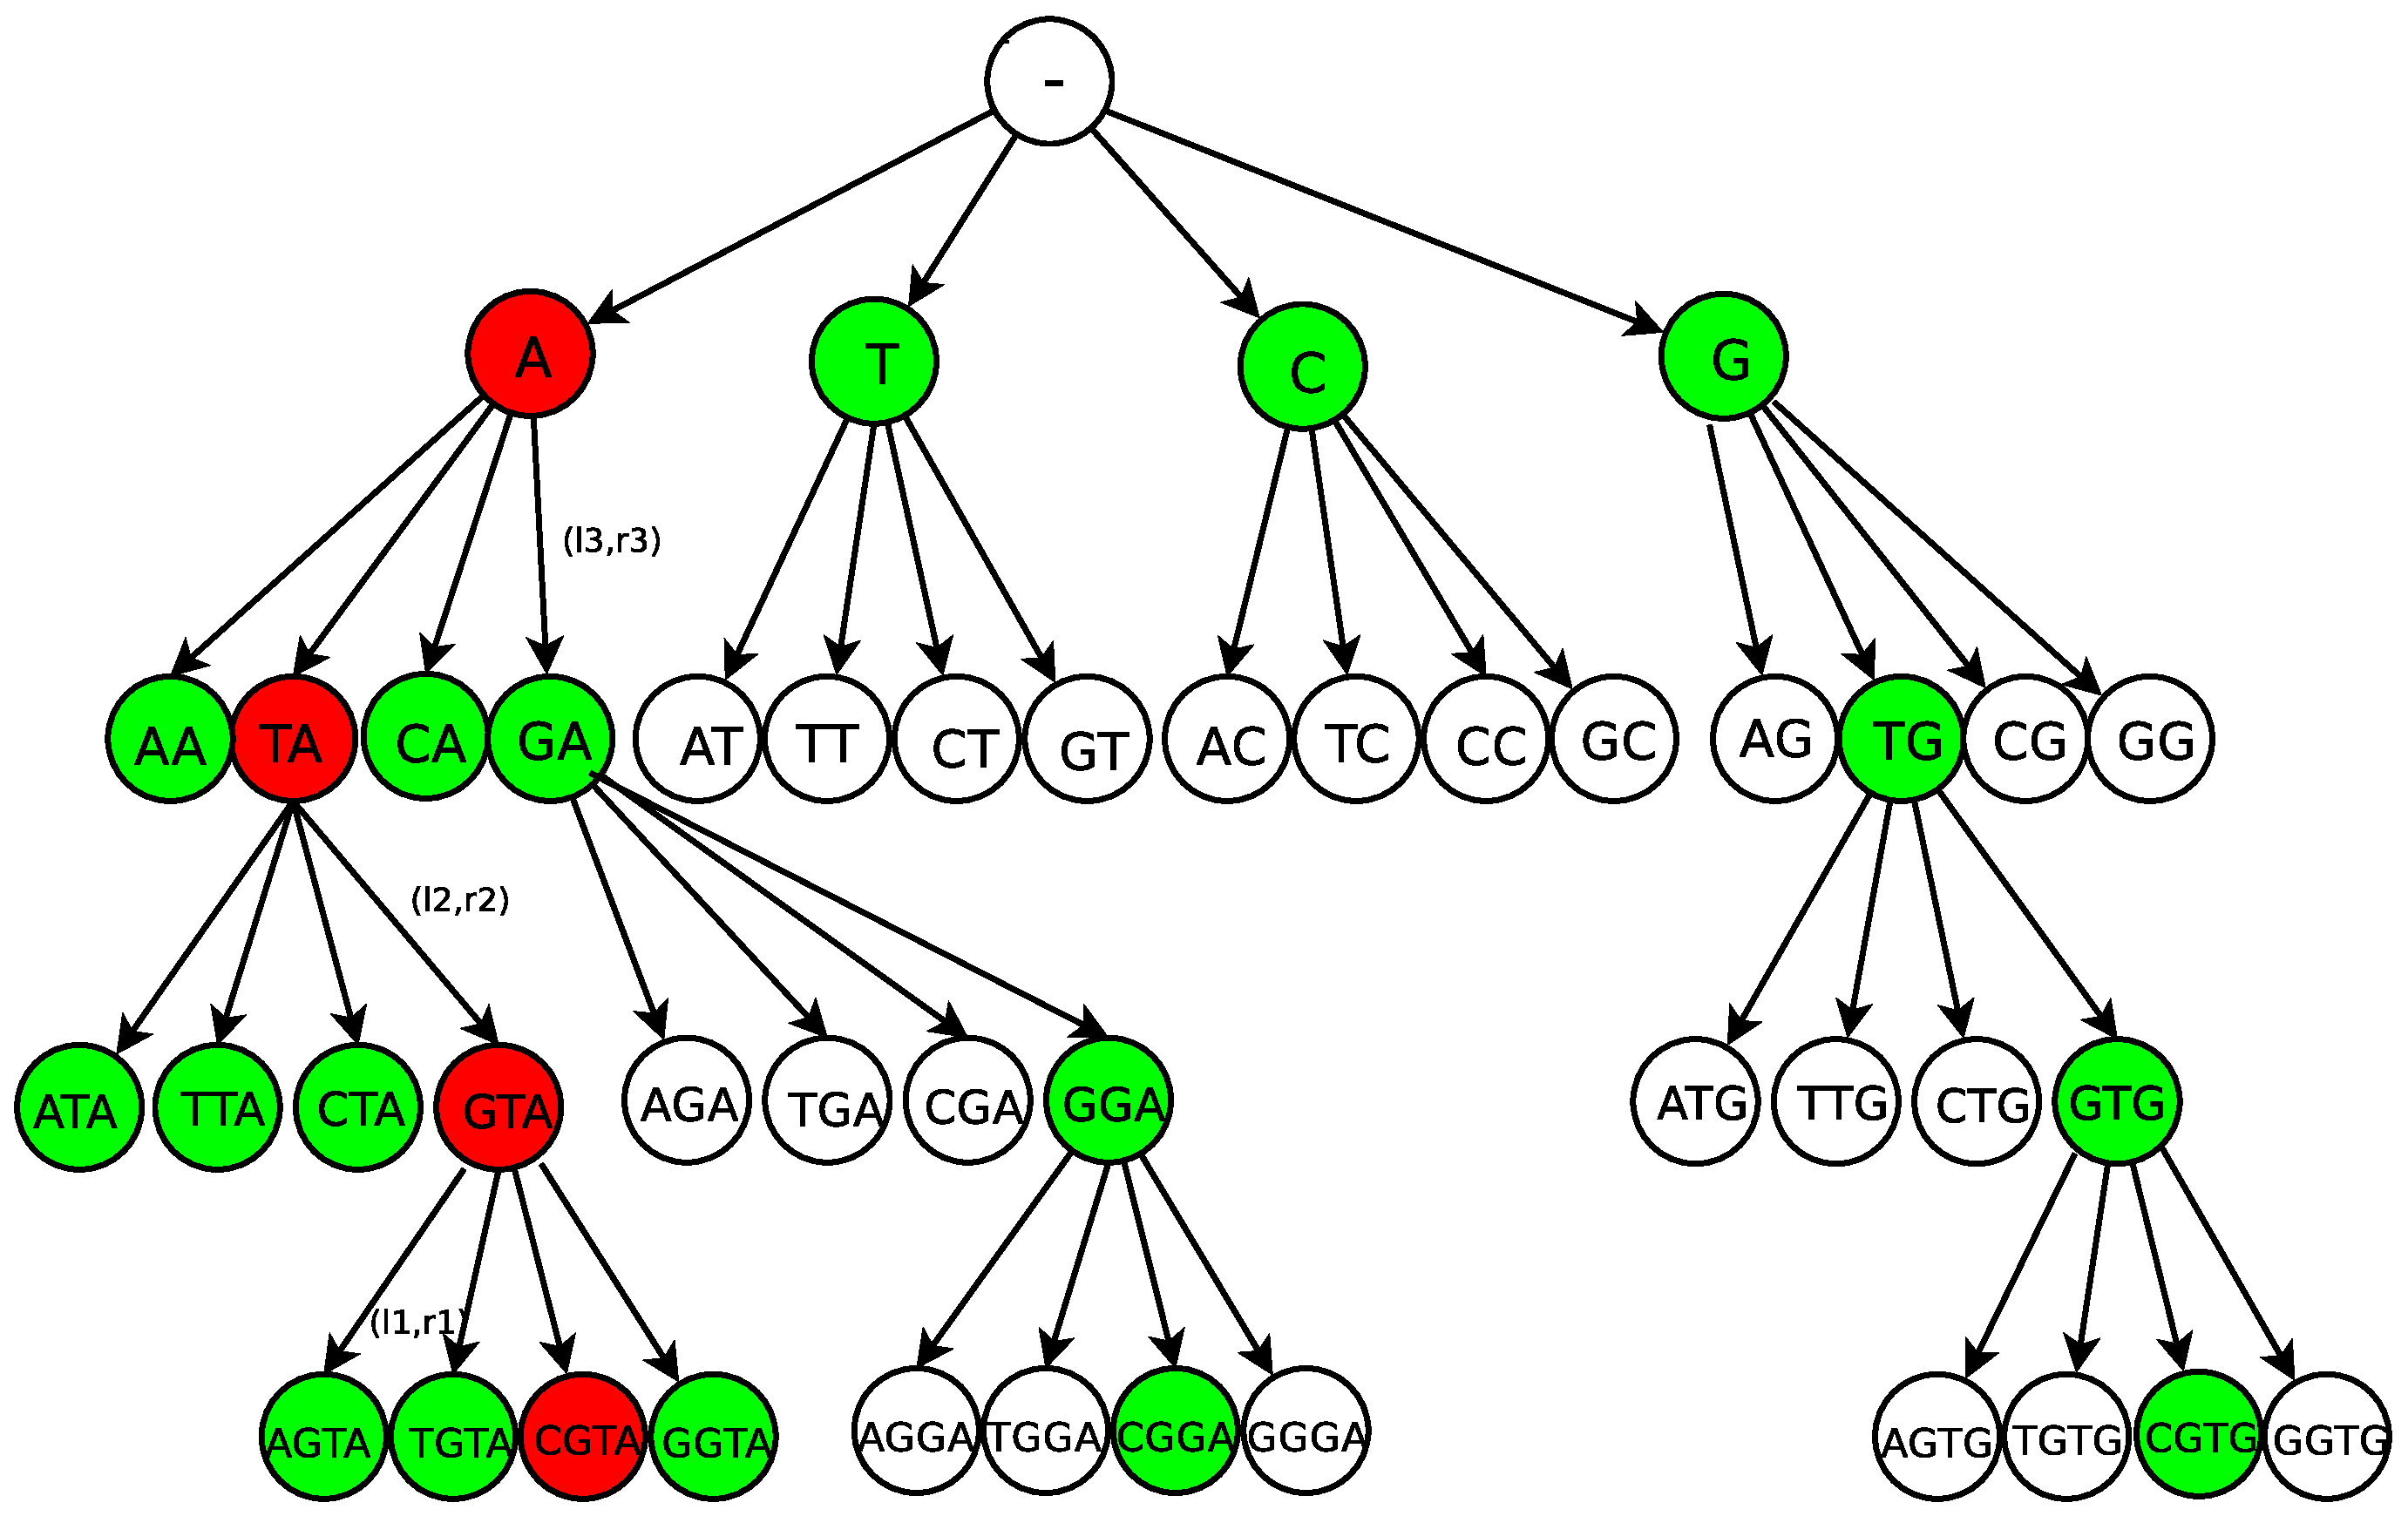
\includegraphics[width=0.9\textwidth]{searchtree.eps}
    \caption{近似匹配示例} \label{fig:searchtree}
\end{figure}

实际上,每一次的替换,删除或者插入操作导致的新的近似序列可以看作一个树上的遍历过程。如图\ref{fig:searchtree}所示,对于一个长
为4的短读 $P=$``CGTA''的搜索过程,简化起见,省略了删除和插入操作。首先通过CSA查询$P[3]=$`A'在参考序列上的后缀数组位置。接着把
$P[3]=$`A'分别替换为`T',`C',`G',在CSA上查找替换后的后缀数组位置。图中红色路径标志的是到当前搜索深度没有替换操作的近似串,而
绿色标记的则是到当前深度有一次替换操作的近似串,无色的是有两次以上替换操作的近似串搜索路径。可以看到,随着搜索深度的增加,搜索
的方向急剧扩大,加上还有未画出的删除和插入操作,可能的搜索方向会更多。

搜索树的本质是对每一个可能的近似序列都进行搜索,假设一个短读序列的长度为$m$,DNA序列字符集为4,根据上一小节,总的时间复杂度为$9^{m-1}+\Theta(m\log n)$。
考虑到$m$一般在20到70之间,如果直接采用搜索树来进行近似匹配,搜索规模会非常大而难以在有效时间内实现。实际上也无需比对所有的近
似串,对于某些替换,删除或者插入操作过多的近似串,应该提前抛弃掉,即采用分支限界法来对搜索树进行剪枝,去除掉无效的搜索方向,降
低搜索空间。

\section{分支限界}

根据上一小节的分析,搜索树的搜索空间复杂度是随短读序列长度指数级增长的,因此必须进行适当的剪枝,抛弃一些没有价值的搜索方向。
传统的DNA序列比对中用到了编辑距离(Edit Distance),汉明距离(Hamming Distance)等来度量两个序列的相似度。在此我们也可以使用类
似的方法做分支限界,比如采用编辑距离,可通过给定一个允许的最大编辑距离$maxDistance$,当在短读序列$P$上后向搜索进行到第$i$步
时,在某个搜索方向上的一个近似序列为$P^{'}$,计算$P$和$P^{'}$之间的编辑距离,若距离大于预先定义的$maxDistance$,则抛弃这个搜
索方向,否则,保持这个搜索方向。汉明距离做分支限界的方法和编辑距离方法类似。

采用编辑距离和汉明距离的方法必须对每一个得到的近似序列和短读序列计算距离,这一方面会导致算法效率的降低,另一方面由于我们在做
短读比对时,会有大量的短读需要比对,这些短读的长度不一定都相同,指定唯一的$maxDistance$是不合适的。对此,在论文\cite{li2009fast}
中,作者提出了一种类似于编辑距离的算法,称之为$difference$数组,该算法很好的实现了自适应的类编辑距离的最大限制距离。因此本文
提出的CSAA比对算法也使用$difference$数组作为分支限界的一个条件。$difference$数组是利用$CSA$上的精确匹配算法,首先对需要比对的
短读做预处理,处理过程如算法\ref{alg:darray}所示。处理过的$difference[i]$反映了在搜索$P[i\ldots n-1]$时可以允许的最大替换,插
入,删除操作的次数。由于在序列比对中我们采用的是后向搜索的过程,所以在计算$difference$数组时,也需要从后往前算,使得$difference$
是一个递减的序列,也即在从后往前比对短读$P[0\ldots n-1]$时,越往前,允许的替换,插入,删除数量越多。

\begin{algorithm}
    \caption{计算$difference$数组}
    \label{alg:darray}
    \begin{algorithmic}[1]
        \Require $\Phi,\alpha,\beta,P$
        \Ensure $difference[0\ldots |P|-1]$
        \Function{CalculateDifference}{$\Phi,\alpha,\beta,P$}
            \State $z \gets 0$
            \State $l \gets 0$
            \State $r \gets |P|-1$
            \For{$i \gets |P|-1$ downto $0$}
                \State $(l,r) \gets$ \Call{ExactMatch}{$\Phi,\alpha,\beta,l,r,P[i]$} \Comment{调用算法\ref{alg:exac}}
                \If {$l>r$}
                \Comment{失配,$difference[i]$增加一次,否则$difference[i]$不变}
                \State $l\gets 0$
                \State $r \gets |P|-1$
                \State $z \gets z+1$
                \EndIf
                \State $difference[i] \gets z$
            \EndFor
        \EndFunction
    \end{algorithmic}
\end{algorithm}

$difference$数组的作用,是结合每一个近似序列的一个辅助值$z$来分支限界的。开始比对时,序列$P$的$z$值是$0$,之后每做一次插入,
删除或者替换,则$z$增加一次,而在该操作位置的最大允许删除,插入,替换操作数是$difference[i]$。比较两者,若$z>difference[i]$
则证明该搜索方向做了过多的替换,删除,插入操作,短读已经和参考序列相似度太小,应当删除该搜索方向,考虑搜索树上的其他方向。

除了$difference$距离,另一可用的分支限界策略是罚分机制\cite{lesk1e21986alignment}。在搜索树上向前搜索时,每一次替换,删除或者插入操作都会产生一个新的近
似序列,而每增加一次这样的操作,都会导致这个方向上的近似序列和参考序列的相似度下降。基于此,我们可以预定义一个罚分上限$maxPenalty$。
同时为替换,插入,删除三种操作分别定义各自的罚分,当这个短读比对过程中每做一次上述操作时,都会对这个近似序列增加相应的罚分,
当罚分达到预定义的最大罚分$maxPenalty$时,即认为这个近似序列已经和短读序列相似度太小,没有必要再继续搜索这个方向。通过这样的
罚分机制,可以去除较差的近似序列,达到分支限界的目的。

在生物信息学领域,每一个删除或者插入统称为一个indel,而每一个indel都会在短读序列上造成一个空位(gap),对应的罚分称为空位罚分。
gap通常分为两种,一种是单独出现在序列中,称为gap open;另一种是连续的gap,称为gap extension。gap open的罚分是各个gap罚分的线
性叠加和,而通常gap extension的罚分不能简单的做线性增加来处理。Affine gap penalties\cite{eddy1998profile}是生物信息学领域常用的一种罚分机制,假设
有一个gap extension长为$x$,则这个gap的罚分为$-(\rho +\sigma x)$,其中$\rho >0$,$\sigma$是每一个indel操作的罚分。

有了$difference$距离和$gap$罚分两种分支限界的策略,可以大大减少搜索的规模,通过控制合适的$maxPenalty$可以实现在比对时间和比对
精度之间的平衡。然而如果直接依赖算法\ref{alg:inexact}实现比对算法也是不合适的。因为算法\ref{alg:inexact}是一个递归的算法,递
归算法本身在实际实现时过于低效,我们的short read一般都长30bp以上,这样的深度是不能用递归的。另一方面,递归比对的本质在
搜索树上表现为一个深度优先的搜索,每一次递归都会把一个方向上的所有方向做一次尝试,直到遇到分支限界条件不合适才会回溯到上一层。
这一特性会引起过度回溯的问题。这一问题的本质是每次进入一个新的搜索方向时没有做出正确的选择,整体的搜索方向是随机的,算法大多
数的递归选择都会进入不是最好的方向,从而最终不得不回溯,这显著增大了时间开销。据此本文提出一种优先堆结构,把搜索树上的深度优
先搜索改为广度优先搜索。每一层上都把所有的搜索方向排序放在一个优先堆里,算法每进入下一个搜索方向都在当前优先堆中选择最优的即
罚分最低的搜索方向进入。借助这一优先堆结构,可以把搜索方向限制在只沿着最优的搜索方向前进,从而实现最优比对。同时,还可以限定
优先堆的大小,抛弃掉虽然符合分支限界条件但相对于其他搜索方向过差的搜索方向。

优先队列使用了最大堆来实现,每一项保存一个近似匹配的序列相关匹配信息,以每个近似序列的罚分和$z$值作为优先堆的$key$值。本文中
使用的优先堆支持如下操作:

\begin{itemize}
    \item INIT-HEAP$(heap)$:初始化优先堆$heap$为空。
    \item INSERT-HEAP$(heap,x)$:把元素$x$插入优先堆$heap$中,并按照罚分排序。
    \item EXTRACT-MIN$(heap)$:去掉并返回$heap$中罚分最小的元素。
    \item HEAP-SIZE$(heap)$:返回$heap$中元素的数量。
    \item HEAP-DROP-MAX$(heap)$:删除$heap$中罚分最大的算素。
\end{itemize}

综上所述,我们提出本文的核心比对算法\ref{alg:alignment},该算法中使用了算法\ref{alg:process},后者是在给定的位置上做替换,
插入,删除操作的过程。比对算法\ref{alg:alignment}可以指定$maxPenalty$和$maxHeapSize$两个参数来控制比对的精度和比对时间之间的
平衡。

\begin{algorithm}
    \caption{处理替换,删除,插入}
    \label{alg:process}
    \begin{algorithmic}[1]
        \Require $P,\Phi,\alpha,\beta,x,heap$
        \Ensure $heap$
        \Function {ProcessIndel}{$P,\Phi,\alpha,\beta,x,heap$}
        \State $y.l\gets x.l$;$y.r\gets x.r$;$y.i\gets x.i-1$  \Comment{删除$P[i]$}
        \State $y.penalty \gets x.penalty+delPenalty$
        \State $y.z\gets x.z+1$
        \State \Call{Insert-Heap}{$heap$,$y$}
        \ForAll{$c \in \{A,C,G,T\}$}
            \State $(l,r)\gets$\Call{ExactMatch}{$\Phi,\alpha,\beta,x.l,x.r,c$}
            \If {$l\leq r$}
                \State $y.l\gets l$;$y.r\gets r$;$y.i\gets x.i$ \Comment{在$P[i]$之后插入$c$}
                \State $y.penalty\gets x.penalty+insPenalty$;
                \State $y.z \gets x.z+1$
                \State \Call{Insert-Heap}{$heap,y$}
                \If {$P[i]=c$}  \Comment{match}
                    \State $y.l\gets l$;$y.r\gets r$;$y.i\gets x.i-1$
                    \State $y.penalty\gets x.penalty$;
                    \State $y.z\gets x.z$
                    \State \Call{Insert-Heap}{$heap,y$}
                \Else   \Comment{替换$P[i]$}
                    \State $y.l\gets l$;$y.r\gets r$;$y.i\gets x.i-1$
                    \State $y.penalty\gets x.penalty+subPenalty$
                    \State $y.z\gets x.z+1$
                    \State \Call{Insert-Heap}{$heap,y$}
                \EndIf
            \EndIf
        \EndFor
        \State \Return $heap$
        \EndFunction
   \end{algorithmic}
\end{algorithm}

\begin{algorithm}
    \caption{CSA比对算法}
    \label{alg:alignment}
    \begin{algorithmic}[1]
        \Require $\Phi,\alpha,\beta,P,maxPenalty,maxHeapSize$
        \Ensure $result$    \Comment{输出为符合比对条件的所有结果组成的优先堆}
        \Function{CSAAlignment}{$\Phi,\alpha,\beta,P,maxPenalty,maxHeapSize$}
        \State $difference\gets$\Call{CalculateDifference}{$\Phi,\alpha,\beta,P$}
        \State $heap \gets$ \Call{Init-Heap}{$heap$}
        \State $result \gets$\Call{Init-Heap}{$result$}
        \State $x.l\gets 0$;$x.r\gets |P|-1$;$x.i\gets |P|-1$
        \State $x.penalty\gets 0$;$x.z\gets 0$
        \State $heap\gets$ \Call{ProcessIndel}{$P,\Phi,\alpha,\beta,x.heap$}    \Comment{处理$P[m-1]$}
        \While{$x\gets$\Call{Extract-Min}{heap}}
            \If {$x.i<0$}
                \State \Call{Insert}{$result,x$}    \Comment{获得一个较好的比对结果}
                \State continue
            \EndIf
            \If{$x.z>difference[x.i]$ or $x.penalty>maxPenalty$}  \Comment{剪枝}
                \State continue
            \EndIf
            \State $heap\gets$\Call{ProcessIndel}{$P,\Phi,\alpha,\beta,x,heap$} \Comment{处理$P[0\ldots m-2]$}
            \While{\Call{Heap-Size}{$heap$}>$maxHeapSize$} \Comment{去除较差的比对方向}
                \State \Call{Heap-Drop-Max}{$heap$}
            \EndWhile
        \EndWhile
        \State \Return $result$    \Comment{返回所有符合条件的比对结果}
        \EndFunction
    \end{algorithmic}
\end{algorithm}

\section {本章小结}
本章是本文的核心,主要介绍了我们提出的序列比对算法比对原理,比对过程,以及对时间,空间占用的分析。首先在第一小节给出了一个简
单的基于压缩后缀数组的精确比对算法,接着在第二小节我们在精确比对的基础上给出了一个理论的递归的近似比对算法。之后我们分析了
近似比对算法的时间和空间需求,提出了分支限界的思想,通过$difference$距离和罚分机制实现了分支限界,最后我们提出了一个实践中
可行的化递归为迭代的优先堆数据结构,提出了最终的比对算法。
